\section{System and Threat Models}
\begin{figure*}[!t]
    \vspace{-15pt}
    \centerline{
    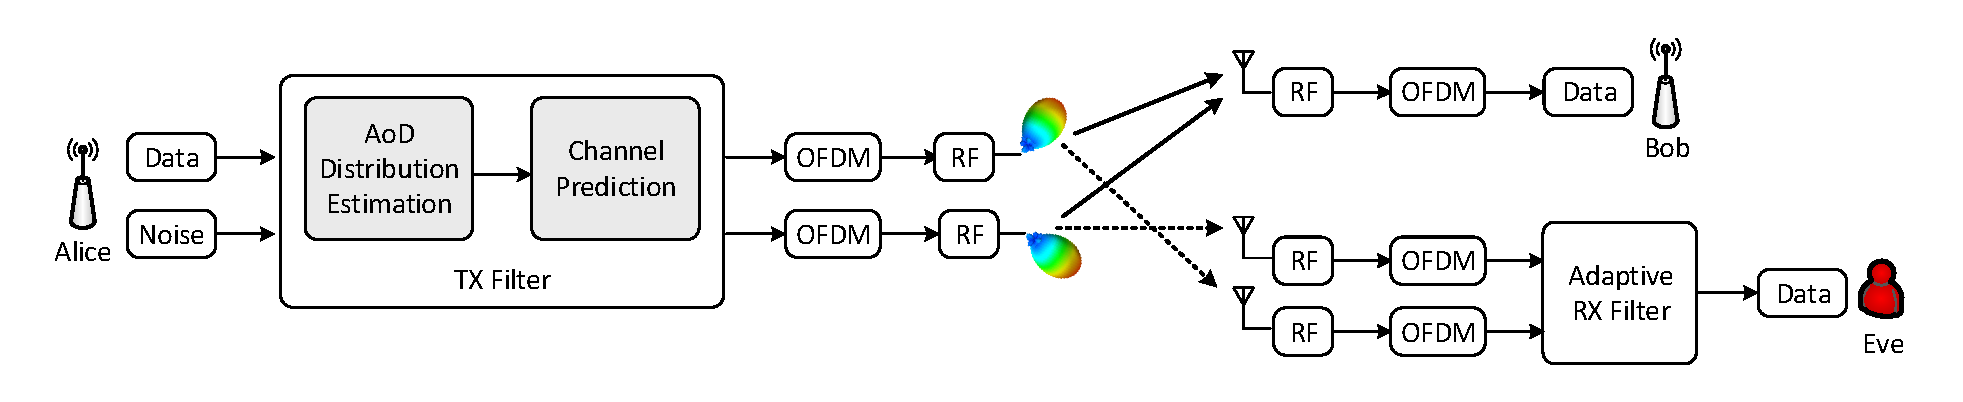
\includegraphics[width=0.8\textwidth]{figs/system.pdf}}
    \caption{Our system model illustrating the transmitter Alice, the legitimate receiver Bob and the passive eavesdropper Eve, where Alice is equipped with RA(s).}
    \label{fig:system}
    \vspace{-15pt}
\end{figure*}

Consider a MIMO-OFDM system shown in Fig. \ref{fig:system}, where the transmitter Alice aims at confidentially communicating with the receiver Bob through a wireless channel $\mathbf{H}_{AB}$, with the existence of a passive eavesdropper Eve. Denote the number of antennas for Alice, Bob and Eve as $n_{a}$, $n_{b}$ and $n_{e}$ respectively. 
The legitimate receiver Bob is equipped with regular omnidirectional antenna(s) (OAs), while the eavesdropper Eve can possess any types of antennas, including OAs, reconfigurable antenna(s) (RAs) and etc.. In particular, the transmitter Alice is equipped with RAs for channel randomization purpose, where an RA is an antenna capable of dynamically reconfiguring its antenna currents or radiating edges in a controlled and reversible manner \cite{bernhard2007reconfigurable}. Typically, an RA can swiftly reconfigurable its antenna profile including radiation pattern, polarization, frequency, and combinations of them. For example, Rodrigo et al. \cite{rodrigo2014frequency} presented an RA that has thousand of antenna modes and can be electronically switched within microseconds. From the receiver's perspective, the effect of the antenna profile is part of the CSI. Hence we can incorporate the impact of RA on the wireless channel into the channel model.

The wireless channel from Alice's $j$-th antenna to a receiver's $i$-th antenna ($(i,j)$-th receive-transmit pair) can be captured by a single complex number in the frequency domain, i.e. $h_{i,j}$, and the full CSI of transceivers can be represented by an array $\mathbf{H}$ with dimension  $n_b \times n_a$. Then the received signal $\mathbf{R}$ with dimension $n_b \times *$ can be expressed as:
\begin{equation}
    \mathbf{R} = \mathbf{H} \cdot \mathbf{D} + \mathbf{N}
\end{equation}
where $\mathbf{D}$ and $\mathbf{N}$ represents the transmitted data and the additive white Gaussian noise (AWGN), with dimension $n_a \times *$ and $n_b \times *$ respectively.
For the channel model, we consider a multipath channel. Recall that the effect of the antenna profile is also part of the CSI, to distinguish, we separate the CSI into the channel coefficient decided by the physical channel itself and the antenna part. Assuming that the channel is composed with $P$ multipaths, denote the physical channel coefficient part of $h_{i,j}$ as $h_{i,j}^{(phy)}$, then
\begin{equation}
    h_{i,j}^{(phy)}=\sum\limits_{l=1}^{P}L_{l}\alpha_{l}e^{-j\phi_{l}}
   \label{eq:h}
\end{equation}
where $L_{l}$ is the path loss of the $l$-th path, and $\alpha_{l}e^{-j\phi_{l}}$ is its fading parameter, here $\alpha_{l}$ and $\phi_{l}$ are the amplitude and phase of the fading respectively. Similar to existing works \cite{anand2012strobe,schulz2014practical,zheng2016profiling}, the physical channel coefficient $ h_{i,j}^{(phy)}$ in our model is fixed during the channel coherent time. Then the multipath channel can be expressed with the distribution of angle-of-departure (AoD). According to the multipath model, a single transmission from the antenna propagates along multiple paths before reaching the receiver. Each signal that travels at a particular AoD along with different paths experiences a different amount of attenuation and phase shifts. Then the physical channel coefficient part expressed as  \eqref{eq:h} can be further extended as the summation of the CSI over all the departure directions, and only the CSI that in the direction of multipaths is non-trivial. The distribution of CSI over all possible AoDs is defined as the AoD distribution. Then,
\begin{equation}
    h_{i,j}^{(phy)}=\sum\limits_{d=1}^{D}\mathbf{a}_{i,j}(\theta_d)
   \label{eq:h2}
\end{equation}
where the angular space is discretized into $D$ unique, equally spaced angles $\{\theta_1,\theta_2, \dots, \theta_D \}$, and $\mathbf{a}_{i,j}$ is the AoD distribution of $(i,j)$-th receive-transmit channel.

With RA, various antenna modes are associated with different radiation patterns. When the antenna gain under antenna mode $u$ and angle-of-departure $\theta_{l}$ is denoted as $\mathbf{G}(u,\theta_d)$, then the CSI $h_{i,j}$ under antenna mode $u$ can written as:
\begin{equation}
  h_{i,j}(u)=\sum\limits_{d=1}^{D}\mathbf{G}(u,\theta_{d})\mathbf{a}_{i,j}(\theta_d)
  \label{eq:hh}
\end{equation}
%and we illustrate this multipath channel model in terms of the AoD distribution with the effect of antennas in Fig. \ref{fig:channel}.

%
%\begin{figure}[t]
%    \vspace{-15pt}
%    \centering
%    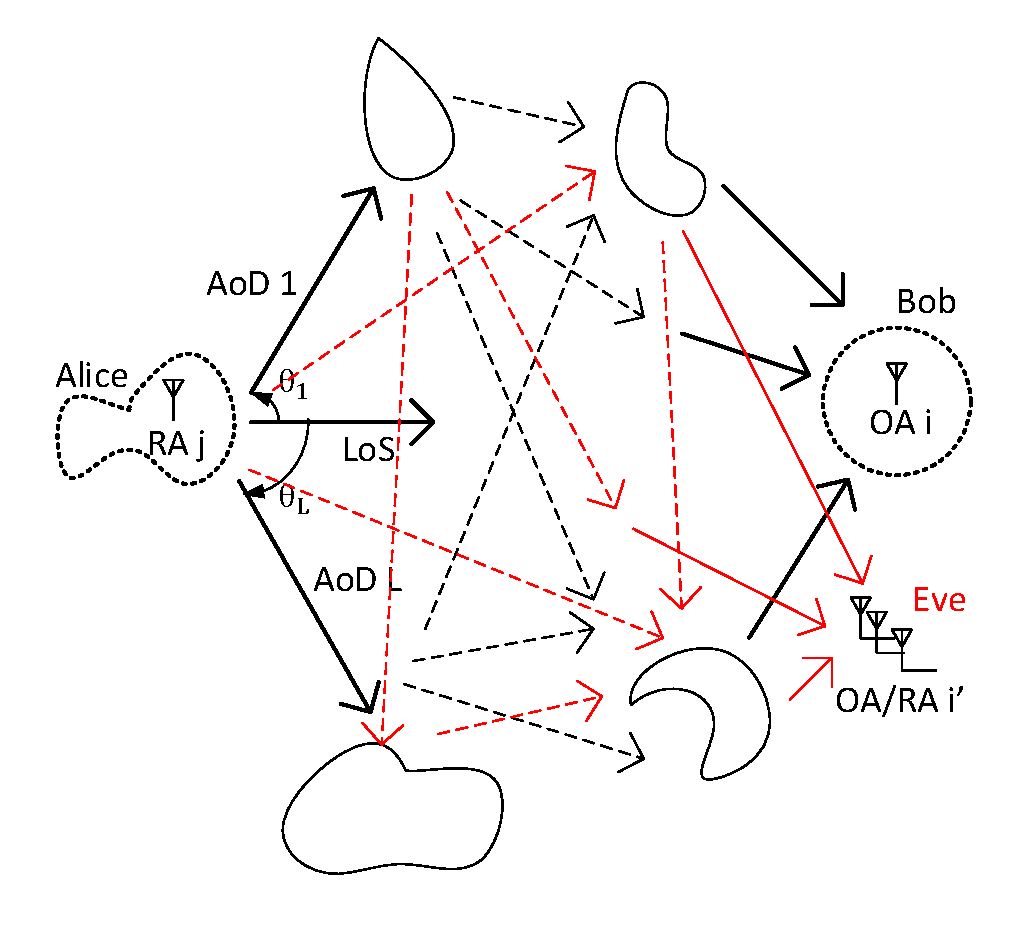
\includegraphics[width=0.3\textwidth]{figs/channel2}
%    \caption{Multipath channel model in terms of the AoD distribution, with the effect of antennas}
%    \label{fig:channel}
%    \vspace{-15pt}
%\end{figure}

% \begin{equation}
%   H_{i,j}=G(u,\theta_{i,j}) \cdot \sum\limits_{l=1}^{P}L_{l}\alpha_{i}e^{-j\phi_{i}}
%   \label{eq:hh}
% \end{equation}

Same as \cite{anand2012strobe,schulz2014practical,zheng2016profiling}, the channel from Alice to Bob ($\mathbf{H}_{AB}$) is measured at Bob's side and can be sent back to Alice through an out-of-band (OOB) channel or rely on implicit feedback, but $\mathbf{H}_{AB}$ is unknown to Eve. And Eve's can measure the channel from Alice to her ($\mathbf{H}_{AE}$), and it is unknown to neither Alice nor Bob. 